\chapter{Word cloud representations}
\label{appendix:word_cloud_representations}

\section{Networks of Topics (Grants as edges)}

\subsection{Based on word frequency}

\begin{figure}[htbp]
    \centering
    \includegraphics[width=\textwidth,height=\textheight,keepaspectratio]{word-clouds/frequency/all}
    \caption[Word cloud representation based on word frequency showcasing words that formulate the topics found in the Topic network (Grants as edges)]{Word cloud representation created using Wordle showcasing words that formulate the topics found in the Topic network (Grants as edges). Font size represents of word frequency within the the text corpus.}
    \label{fig:topic_grant_freq_all}
\end{figure}

\subsection{Based on the number of grants containing topics}

\begin{figure}[htbp]
    \centering
    \includegraphics[width=\textwidth,height=\textheight,keepaspectratio]{word-clouds/number/all}
    \caption[Word cloud representation based on the number of grants containing topics found in the Topic network (Grants as edges)]{Word cloud representation created using Wordle showcasing topics found in the Topic network (Grants as edges). Font size represents the number of grants containing a specific topic.}
    \label{fig:topic_grant_number_all}
\end{figure}

\clearpage

\subsection{Based on the value of grants containing topics}

\begin{figure}[htbp]
    \centering
    \includegraphics[width=\textwidth,height=\textheight,keepaspectratio]{word-clouds/value/all}
    \caption[Word cloud representation based on the value of grants containing topics found in the Topic network (Grants as edges)]{Word cloud representation created using Wordle showcasing topics topics found in the Topic network (Grants as edges). Font size represents the number of grants containing a specific topic.}
    \label{fig:topic_grant_value_all}
\end{figure}

\section{Communities of topics}

\subsection{Community 1}

\subsubsection{Based on word frequency}

\begin{figure}[htbp]
    \centering
    
\includegraphics[width=\textwidth,height=\textheight,keepaspectratio]{word-clouds/frequency/c1}
    \caption[Word cloud representation based on word frequency showcasing words that formulate the topics clustered within Community 1]{Word cloud representation created using Wordle showcasing words that formulate the topics clustered within Community 1 as identified by the Louvain community detection algorithm. Font size represents the frequency of the word in the text corpus made out of all the words that formulate the topics clustered in Community 1.}
    \label{fig:topic_grant_freq_c1_appendix}
\end{figure}

\clearpage

\subsubsection{Based on the number of grants containing topics}

\begin{figure}[htbp]
    \centering
    
\includegraphics[width=\textwidth,height=\textheight,keepaspectratio]{word-clouds/number/c1}
    \caption[Word cloud representation based on the number of grants containing topics clustered within Community 1]{Word cloud representation created using Wordle showcasing topics clustered within Community 1 as identified by the Louvain community detection algorithm. Font size represents the number of grants containing a specific topic.}
    \label{fig:topic_grant_number_c1_appendix}
\end{figure}

\subsubsection{Based on the value of grants containing topics}

\begin{figure}[!htbp]
    \centering
    
\includegraphics[width=\textwidth,height=\textheight,keepaspectratio]{word-clouds/value/c1}
    \caption[Word cloud representation based on the value of grants containing topics clustered within Community 1]{Word cloud representation created using Wordle showcasing topics clustered within Community 1 as identified by the Louvain community detection algorithm. Font size represents the number of grants containing a specific topic.}
    \label{fig:topic_grant_value_c1_appendix}
\end{figure}

\clearpage

\subsection{Community 2}

\subsubsection{Based on word frequency}

\begin{figure}[htbp]
    \centering
    \includegraphics[width=\textwidth,height=\textheight,keepaspectratio]{word-clouds/frequency/c2}
    \caption[Word cloud representation based on word frequency showcasing words that formulate the topics clustered within Community 2]{Word cloud representation created using Wordle showcasing words that formulate the topics clustered within Community 2 as identified by the Louvain community detection algorithm. Font size represents the frequency of the word in the text corpus made out of all the words that formulate the topics clustered in Community 2.}
    \label{fig:topic_grant_freq_c2}
\end{figure}

\subsubsection{Based on the number of grants containing topics}

\begin{figure}[htbp]
    \centering
    \includegraphics[width=\textwidth,height=\textheight,keepaspectratio]{word-clouds/number/c2}
    \caption[Word cloud representation based on the number of grants containing topics clustered within Community 2]{Word cloud representation created using Wordle showcasing topics clustered within Community 2 as identified by the Louvain community detection algorithm. Font size represents the number of grants containing a specific topic.}
    \label{fig:topic_grant_number_c2}
\end{figure}

\clearpage

\subsubsection{Based on the value of grants containing topics}

\begin{figure}[htbp]
    \centering
    \includegraphics[width=\textwidth,height=\textheight,keepaspectratio]{word-clouds/value/c2}
    \caption[Word cloud representation based on the value of grants containing topics clustered within Community 2]{Word cloud representation created using Wordle showcasing topics clustered within Community 2 as identified by the Louvain community detection algorithm. Font size represents the number of grants containing a specific topic.}
    \label{fig:topic_grant_value_c2}
\end{figure}

\subsection{Community 3}

\subsubsection{Based on word frequency}

\begin{figure}[htbp]
    \centering
    \includegraphics[width=\textwidth,height=\textheight,keepaspectratio]{word-clouds/frequency/c3}
    \caption[Word cloud representation based on word frequency showcasing words that formulate the topics clustered within Community 3]{Word cloud representation created using Wordle showcasing words that formulate the topics clustered within Community 1 as identified by the Louvain community detection algorithm. Font size represents the frequency of the word in the text corpus made out of all the words that formulate the topics clustered in Community 3.}
    \label{fig:topic_grant_freq_c3}
\end{figure}

\clearpage

\subsubsection{Based on the number of grants containing topics}

\begin{figure}[htbp]
    \centering
    \includegraphics[width=\textwidth,height=\textheight,keepaspectratio]{word-clouds/number/c3}
    \caption[Word cloud representation based on the number of grants containing topics clustered within Community 3]{Word cloud representation created using Wordle showcasing topics clustered within Community 3 as identified by the Louvain community detection algorithm. Font size represents the number of grants containing a specific topic.}
    \label{fig:topic_grant_number_c3}
\end{figure}

\subsubsection{Based on the value of grants containing topics}

\begin{figure}[htbp]
    \centering
    \includegraphics[width=\textwidth,height=\textheight,keepaspectratio]{word-clouds/value/c3}
    \caption[Word cloud representation based on the value of grants containing topics clustered within Community 3]{Word cloud representation created using Wordle showcasing topics clustered within Community 3 as identified by the Louvain community detection algorithm. Font size represents the number of grants containing a specific topic.}
    \label{fig:topic_grant_value_c3}
\end{figure}

\clearpage

\subsection{Community 4}

\subsubsection{Based on word frequency}

\begin{figure}[htbp]
    \centering
    \includegraphics[width=\textwidth,height=\textheight,keepaspectratio]{word-clouds/frequency/c4}
    \caption[Word cloud representation based on word frequency showcasing words that formulate the topics clustered within Community 4]{Word cloud representation created using Wordle showcasing words that formulate the topics clustered within Community 4 as identified by the Louvain community detection algorithm. Font size represents the frequency of the word in the text corpus made out of all the words that formulate the topics clustered in Community 4.}
    \label{fig:topic_grant_freq_c4}
\end{figure}

\subsubsection{Based on the number of grants containing topics}

\begin{figure}[htbp]
    \centering
    \includegraphics[width=\textwidth,height=\textheight,keepaspectratio]{word-clouds/number/c4}
    \caption[Word cloud representation based on the number of grants containing topics clustered within Community 4]{Word cloud representation created using Wordle showcasing topics clustered within Community 4 as identified by the Louvain community detection algorithm. Font size represents the number of grants containing a specific topic.}
    \label{fig:topic_grant_number_c4}
\end{figure}

\clearpage

\subsubsection{Based on the value of grants containing topics}

\begin{figure}[htbp]
    \centering
    \includegraphics[width=\textwidth,height=\textheight,keepaspectratio]{word-clouds/value/c4}
    \caption[Word cloud representation based on the value of grants containing topics clustered within Community 4]{Word cloud representation created using Wordle showcasing topics clustered within Community 4 as identified by the Louvain community detection algorithm. Font size represents the number of grants containing a specific topic.}
    \label{fig:topic_grant_value_c4}
\end{figure}

\subsection{Community 5}

\subsubsection{Based on word frequency}

\begin{figure}[htbp]
    \centering
    \includegraphics[width=\textwidth,height=\textheight,keepaspectratio]{word-clouds/frequency/c5}
    \caption[Word cloud representation based on word frequency showcasing words that formulate the topics clustered within Community 5]{Word cloud representation created using Wordle showcasing words that formulate the topics clustered within Community 5 as identified by the Louvain community detection algorithm. Font size represents the frequency of the word in the text corpus made out of all the words that formulate the topics clustered in Community 5.}
    \label{fig:topic_grant_freq_c5}
\end{figure}

\clearpage

\subsubsection{Based on the number of grants containing topics}

\begin{figure}[htbp]
    \centering
    \includegraphics[width=\textwidth,height=\textheight,keepaspectratio]{word-clouds/number/c5}
    \caption[Word cloud representation based on the number of grants containing topics clustered within Community 5]{Word cloud representation created using Wordle showcasing topics clustered within Community 5 as identified by the Louvain community detection algorithm. Font size represents the number of grants containing a specific topic.}
    \label{fig:topic_grant_number_c5}
\end{figure}

\subsubsection{Based on the value of grants containing topics}

\begin{figure}[htbp]
    \centering
    \includegraphics[width=\textwidth,height=\textheight,keepaspectratio]{word-clouds/value/c5}
    \caption[Word cloud representation based on the value of grants containing topics clustered within Community 5]{Word cloud representation created using Wordle showcasing topics clustered within Community 5 as identified by the Louvain community detection algorithm. Font size represents the number of grants containing a specific topic.}
    \label{fig:topic_grant_value_c5}
\end{figure}

\clearpage

\subsection{Community 6}

\subsubsection{Based on word frequency}

\begin{figure}[htbp]
    \centering
    \includegraphics[width=\textwidth,height=\textheight,keepaspectratio]{word-clouds/frequency/c6}
    \caption[Word cloud representation based on word frequency showcasing words that formulate the topics clustered within Community 6]{Word cloud representation created using Wordle showcasing words that formulate the topics clustered within Community 6 as identified by the Louvain community detection algorithm. Font size represents the frequency of the word in the text corpus made out of all the words that formulate the topics clustered in Community 6.}
    \label{fig:topic_grant_freq_c6}
\end{figure}

\subsubsection{Based on the number of grants containing topics}

\begin{figure}[htbp]
    \centering
    \includegraphics[width=\textwidth,height=\textheight,keepaspectratio]{word-clouds/number/c6}
    \caption[Word cloud representation based on the number of grants containing topics clustered within Community 6]{Word cloud representation created using Wordle showcasing topics clustered within Community 6 as identified by the Louvain community detection algorithm. Font size represents the number of grants containing a specific topic.}
    \label{fig:topic_grant_number_c6}
\end{figure}

\clearpage

\subsubsection{Based on the value of grants containing topics}

\begin{figure}[htbp]
    \centering
    \includegraphics[width=\textwidth,height=\textheight,keepaspectratio]{word-clouds/value/c6}
    \caption[Word cloud representation based on the value of grants containing topics clustered within Community 6]{Word cloud representation created using Wordle showcasing topics clustered within Community 6 as identified by the Louvain community detection algorithm. Font size represents the number of grants containing a specific topic.}
    \label{fig:topic_grant_value_c6}
\end{figure}

\section{Sub-communities of topics}

\subsection{Sub-communities within Community 1}

\subsubsection{Based on the number of grants containing topics}

\begin{figure}[htbp]
    \centering
    \includegraphics[width=\textwidth,height=\textheight,keepaspectratio]{word-clouds/number/sc1}
    \caption[Word cloud representation based on the number of grants containing topics in sub-communities within Community 1]{Word cloud representation showcasing topics in sub-communities within Community 1 as identified by the Louvain community detection algorithm. Font size represents the number of grants containing a specific topic, while text colour represents the sub-communities identified within Community 1.}
    \label{fig:topic_grant_number_sc1}
\end{figure}

\clearpage

\subsubsection{Based on the value of grants containing topics}

\begin{figure}[htbp]
    \centering
    \includegraphics[width=\textwidth,height=\textheight,keepaspectratio]{word-clouds/value/sc1}
    \caption[Word cloud representation based on the value of grants containing topics in sub-communities within Community 1]{Word cloud representation showcasing topics in sub-communities within Community 1 as identified by the Louvain community detection algorithm. Font size represents the value of grants containing a specific topic, while text colour represents the sub-communities identified within Community 1.}
    \label{fig:topic_grant_value_sc1}
\end{figure}

\subsection{Sub-communities within Community 2}

\subsubsection{Based on the number of grants containing topics}

\begin{figure}[htbp]
    \centering
    \includegraphics[width=\textwidth,height=\textheight,keepaspectratio]{word-clouds/number/sc2}
    \caption[Word cloud representation based on the number of grants containing topics in sub-communities within Community 2]{Word cloud representation showcasing topics in sub-communities within Community 2 as identified by the Louvain community detection algorithm. Font size represents the number of grants containing a specific topic, while text colour represents the sub-communities identified within Community 2.}
    \label{fig:topic_grant_number_sc2}
\end{figure}

\clearpage

\subsubsection{Based on the value of grants containing topics}

\begin{figure}[htbp]
    \centering
    \includegraphics[width=\textwidth,height=\textheight,keepaspectratio]{word-clouds/value/sc2}
    \caption[Word cloud representation based on the value of grants containing topics in sub-communities within Community 2]{Word cloud representation showcasing topics in sub-communities within Community 2 as identified by the Louvain community detection algorithm. Font size represents the value of grants containing a specific topic, while text colour represents the sub-communities identified within Community 2.}
    \label{fig:topic_grant_value_sc2}
\end{figure}

\subsection{Sub-communities within Community 3}

\subsubsection{Based on the number of grants containing topics}

\begin{figure}[htbp]
    \centering
    \includegraphics[width=\textwidth,height=\textheight,keepaspectratio]{word-clouds/number/sc3}
    \caption[Word cloud representation based on the number of grants containing topics in sub-communities within Community 3]{Word cloud representation showcasing topics in sub-communities within Community 3 as identified by the Louvain community detection algorithm. Font size represents the number of grants containing a specific topic, while text colour represents the sub-communities identified within Community 3.}
    \label{fig:topic_grant_number_sc3}
\end{figure}

\subsubsection{Based on the value of grants containing topics}

\begin{figure}[htbp]
    \centering
    \includegraphics[width=\textwidth,height=\textheight,keepaspectratio]{word-clouds/value/sc3}
    \caption[Word cloud representation based on the value of grants containing topics in sub-communities within Community 3]{Word cloud representation showcasing topics in sub-communities within Community 3 as identified by the Louvain community detection algorithm. Font size represents the value of grants containing a specific topic, while text colour represents the sub-communities identified within Community 3.}
    \label{fig:topic_grant_value_sc3}
\end{figure}

\subsection{Sub-communities within Community 4}

\subsubsection{Based on the number of grants containing topics}

\begin{figure}[htbp]
    \centering
    \includegraphics[width=\textwidth,height=\textheight,keepaspectratio]{word-clouds/number/sc4}
    \caption[Word cloud representation based on the number of grants containing topics in sub-communities within Community 4]{Word cloud representation showcasing topics in sub-communities within Community 4 as identified by the Louvain community detection algorithm. Font size represents the number of grants containing a specific topic, while text colour represents the sub-communities identified within Community 4.}
    \label{fig:topic_grant_number_sc4}
\end{figure}

\clearpage

\subsubsection{Based on the value of grants containing topics}

\begin{figure}[htbp]
    \centering
    \includegraphics[width=\textwidth,height=\textheight,keepaspectratio]{word-clouds/value/sc4}
    \caption[Word cloud representation based on the value of grants containing topics in sub-communities within Community 4]{Word cloud representation showcasing topics in sub-communities within Community 4 as identified by the Louvain community detection algorithm. Font size represents the value of grants containing a specific topic, while text colour represents the sub-communities identified within Community 4.}
    \label{fig:topic_grant_value_sc4}
\end{figure}

\subsection{Sub-communities within Community 5}

\subsubsection{Based on the number of grants containing topics}

\begin{figure}[htbp]
    \centering
    \includegraphics[width=\textwidth,height=\textheight,keepaspectratio]{word-clouds/number/sc5}
    \caption[Word cloud representation based on the number of grants containing topics in sub-communities within Community 5]{Word cloud representation showcasing topics in sub-communities within Community 5 as identified by the Louvain community detection algorithm. Font size represents the number of grants containing a specific topic, while text colour represents the sub-communities identified within Community 5.}
    \label{fig:topic_grant_number_sc5}
\end{figure}

\clearpage

\subsubsection{Based on the value of grants containing topics}

\begin{figure}[htbp]
    \centering
    \includegraphics[width=\textwidth,height=\textheight,keepaspectratio]{word-clouds/value/sc5}
    \caption[Word cloud representation based on the value of grants containing topics in sub-communities within Community 5]{Word cloud representation showcasing topics in sub-communities within Community 5 as identified by the Louvain community detection algorithm. Font size represents the value of grants containing a specific topic, while text colour represents the sub-communities identified within Community 5.}
    \label{fig:topic_grant_value_sc5}
\end{figure}

\subsection{Sub-communities within Community 6}

\subsubsection{Based on the number of grants containing topics}

\begin{figure}[htbp]
    \centering
    \includegraphics[width=\textwidth,height=\textheight,keepaspectratio]{word-clouds/number/sc6}
    \caption[Word cloud representation based on the number of grants containing topics in sub-communities within Community 6]{Word cloud representation showcasing topics in sub-communities within Community 6 as identified by the Louvain community detection algorithm. Font size represents the number of grants containing a specific topic, while text colour represents the sub-communities identified within Community 6.}
    \label{fig:topic_grant_number_sc6}
\end{figure}

\clearpage

\subsubsection{Based on the value of grants containing topics}

\begin{figure}[htbp]
    \centering
    \includegraphics[width=\textwidth,height=\textheight,keepaspectratio]{word-clouds/value/sc6}
    \caption[Word cloud representation based on the value of grants containing topics in sub-communities within Community 6]{Word cloud representation showcasing topics in sub-communities within Community 6 as identified by the Louvain community detection algorithm. Font size represents the value of grants containing a specific topic, while text colour represents the sub-communities identified within Community 6.}
    \label{fig:topic_grant_value_sc6}
\end{figure}